\section{The Journey}
\label{app:journey}
\begin{figure}[htbp]
  \centering
  \begin{subfigure}[t]{0.32\linewidth}\centering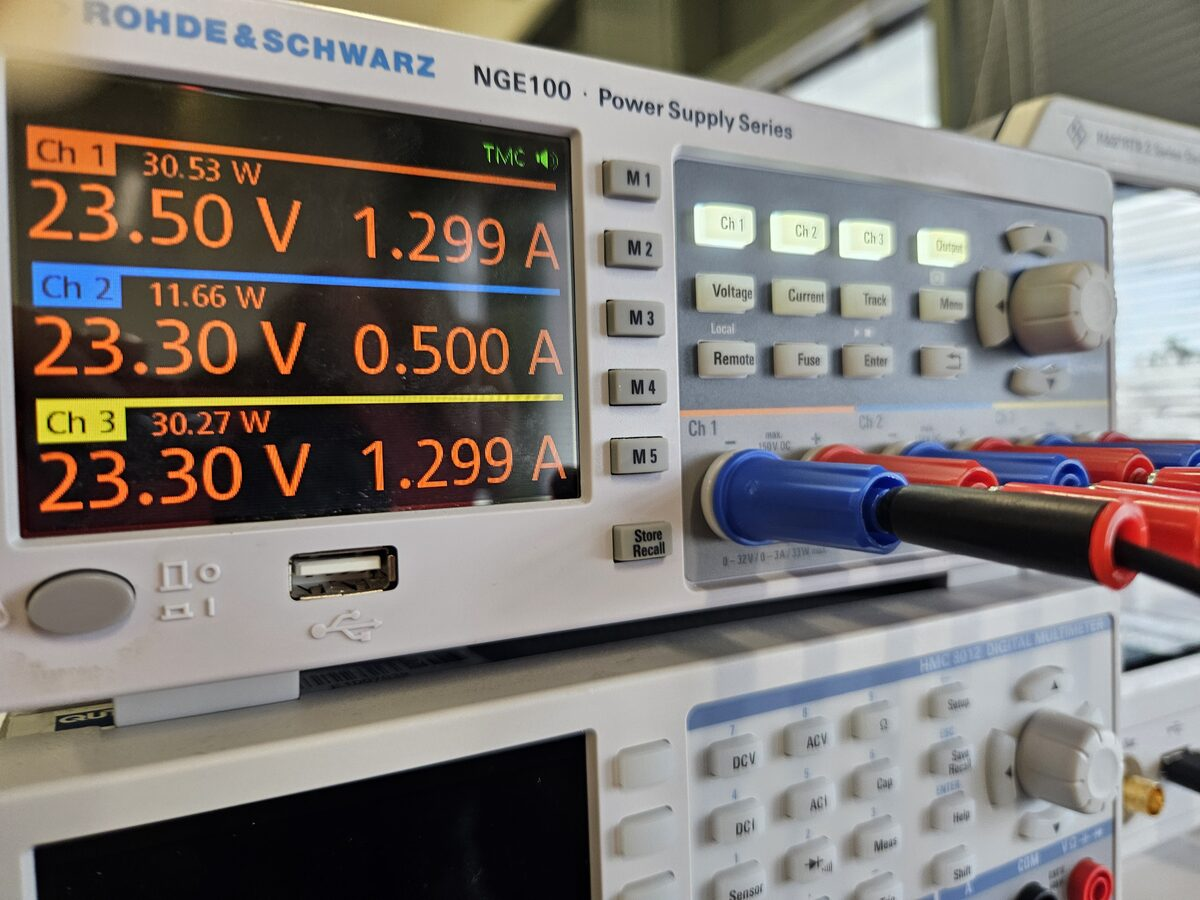
\includegraphics[width=\linewidth,height=3.4cm,keepaspectratio]{20261016_143219}\caption{NGE103 PSU: 23.30\,V / 1.299\,A, 23.30\,V / 0.500\,A, 23.30\,V / 1.299\,A.}\end{subfigure}\hfill
  \begin{subfigure}[t]{0.32\linewidth}\centering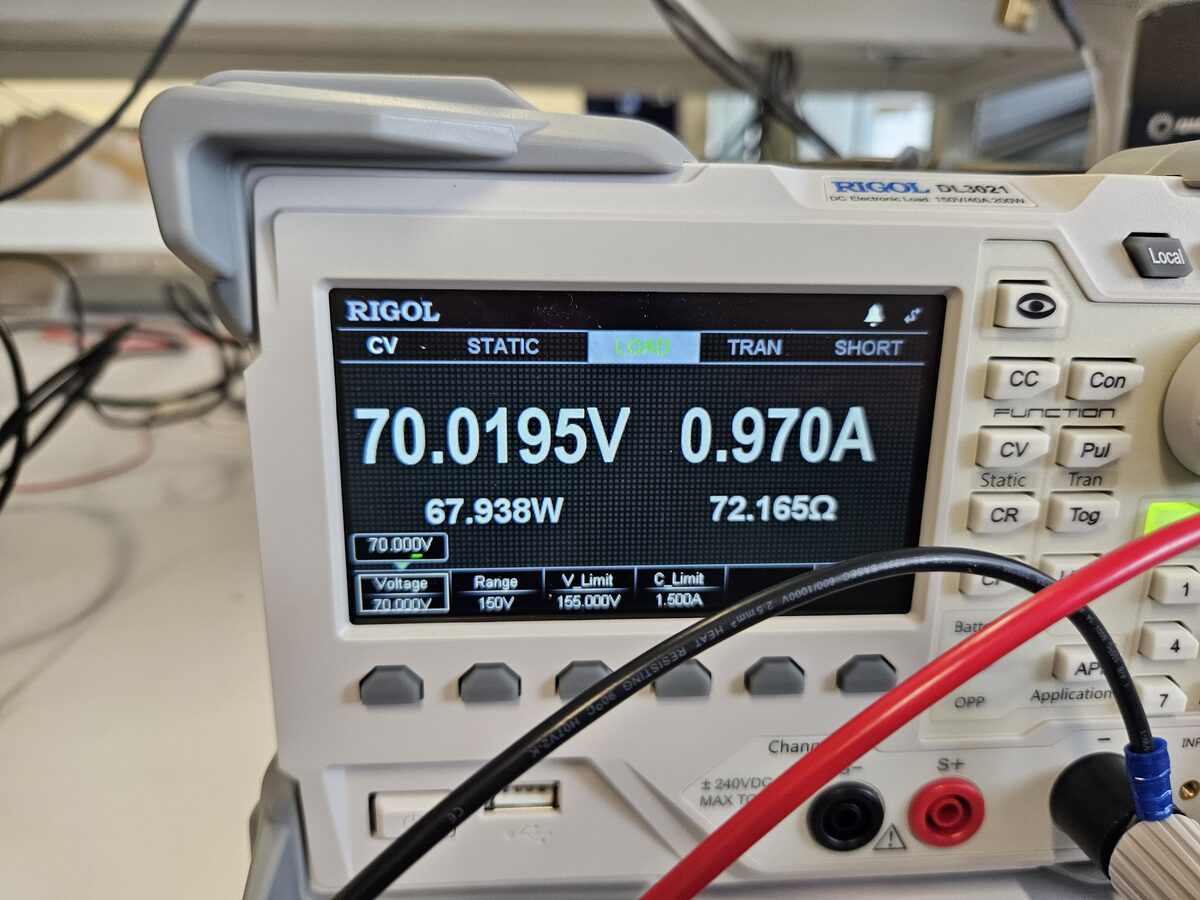
\includegraphics[width=\linewidth,height=3.4cm,keepaspectratio]{20261016_143227}\caption{DL3021 e-load in CV: 70.02\,V, 0.970\,A, 67.9\,W.}\end{subfigure}\hfill
  \begin{subfigure}[t]{0.32\linewidth}\centering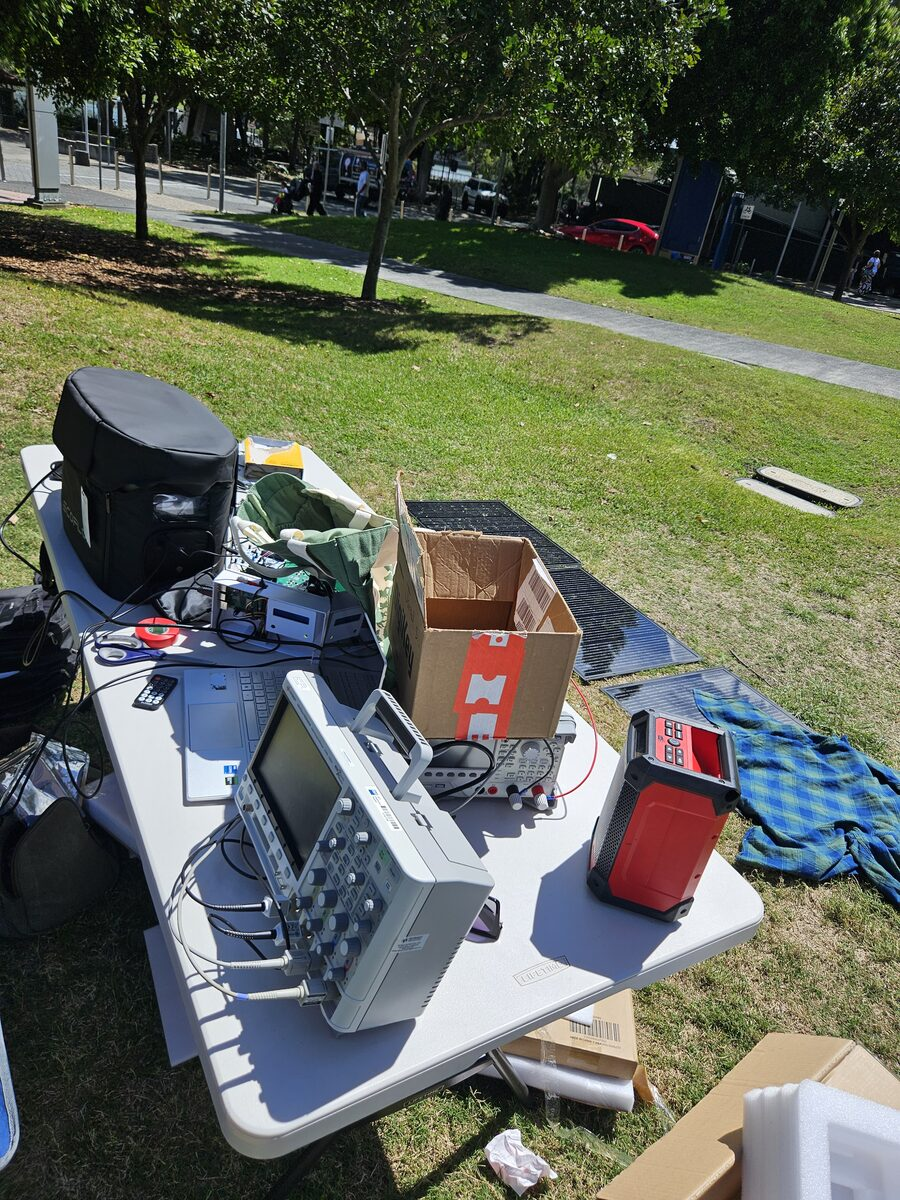
\includegraphics[width=\linewidth,height=3.4cm,keepaspectratio]{20261020_132132}\caption{Carpark string on 20 Oct 2026.}\end{subfigure}
  \caption[{Photographs of the two set-ups}]{Photographs of the two set-ups (more in \cref{app:journey}).}
  \label{fig:setupphotos}
\end{figure}
\newcommand{\ph}[2]{\begin{subfigure}[t]{0.32\linewidth}\centering\includegraphics[width=\linewidth,height=4.6cm,keepaspectratio]{#1}\caption{#2}\end{subfigure}}
\begin{figure}[htbp]
  \centering
  \ph{20260828_075344}{Aug: first proto-board with the Nucleo.}\hfill
  \ph{20260925_000522}{Sep: the Version 0 PCB arrives.}\hfill
  \ph{20261004_141445}{Oct 4: reflow in the PCB oven.}\\[3pt]
  \ph{20261004_162523}{Oct 4: assembled board with the Nucleo.}\hfill
  \ph{20261004_162616}{Oct 4: the hardware teammate with the board.}\hfill
  \ph{20261006_102236}{Oct 6: heatsink.}\\[3pt]
  \ph{20261007_081025}{Oct 7: enclosure work.}\hfill
  \ph{20261011_101108}{Oct 11: pod with the Pi, LCD and IR receiver.}\hfill
  \ph{20261014_100557}{Oct 14: heatsink mounted, thermal paste.}
  \caption{Build photographs (1 of 2).}
\end{figure}
\begin{figure}[htbp]
  \centering
  \ph{20261014_164518}{Oct 14: U10, the top INA239 behind the reversed isolator.}\hfill
  \ph{20261014_212624}{Oct 14: ERUC23 coupled inductor rework.}\hfill
  \ph{20261012_180815}{Oct 12: first bench runs.}\\[3pt]
  \ph{20261016_143209}{Oct 16: pod LCD during the bench test.}\hfill
  \ph{20261016_153331}{Oct 16: Grafana live during closed loop.}\hfill
  \ph{IMG-20261014}{Oct 14: late-night bring-up.}\\[3pt]
  \ph{20261020_131748}{Oct 20: carpark set-up.}\hfill
  \ph{20261020_131809}{Oct 20: it works in the sun.}\hfill
  \ph{20261020_132132}{Oct 20: the string.}
  \caption[{Build and test photographs (2 of 2)}]{Build and test photographs (2 of 2). Videos of the bench runs are in the project repository.}
\end{figure}
